\documentclass{article}
\usepackage[shortlabels]{enumitem}
\usepackage[utf8]{inputenc}
\usepackage{amsmath}
\usepackage{amssymb}
\usepackage{amsthm}
\usepackage{cancel}
\usepackage{graphicx}
\usepackage[top=0.5in, bottom=0.5in, left=1in, right=1in]{geometry}
\usepackage{float}

\title{\textbf{\underline{CSCI 4030U: Big Data Analytics}\\\vspace{5pt}Labs 4 and 5}}
\author{Syed Naqvi\\100590852}
\date{\today}

\begin{document}

    \maketitle
    
    \subsection*{Lab 4} 

    \begin{enumerate}[label=\alph*., left=10pt, itemsep=10pt]

        \item \begin{minipage}[t]{0.9\textwidth}
            Limiting the Apriori algorithm to only find up to frequent pairs:
            \begin{figure}[H]
                \centering
                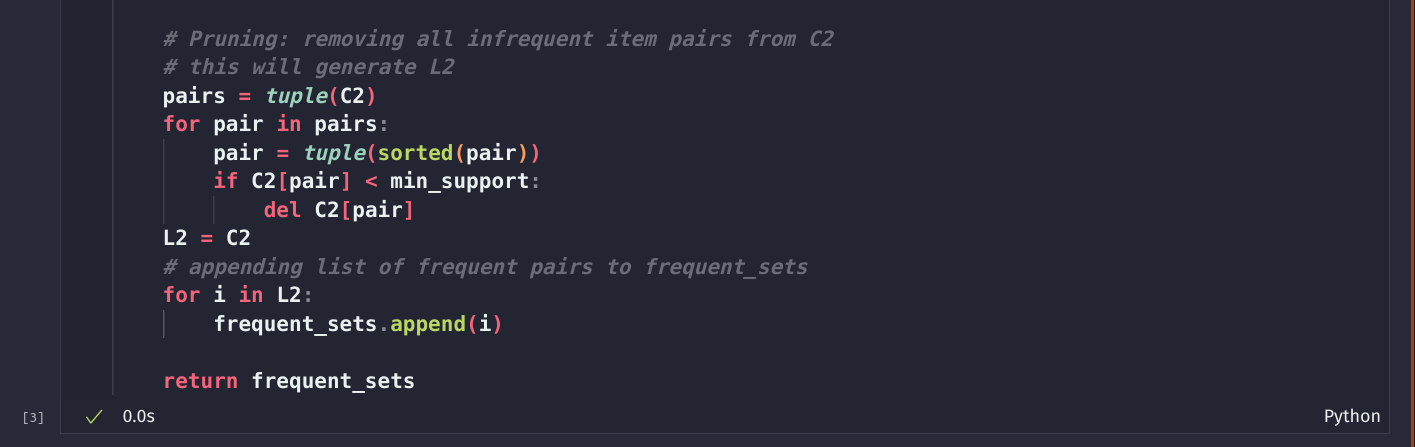
\includegraphics[width=1\textwidth, height=0.2\textheight]{./a.png}
            \end{figure}
        \end{minipage}

        \item \begin{minipage}[t]{0.9\textwidth}
            Downloading retail dataset for the PCY and Apriori algorithms:
            \begin{figure}[H]
                \centering
                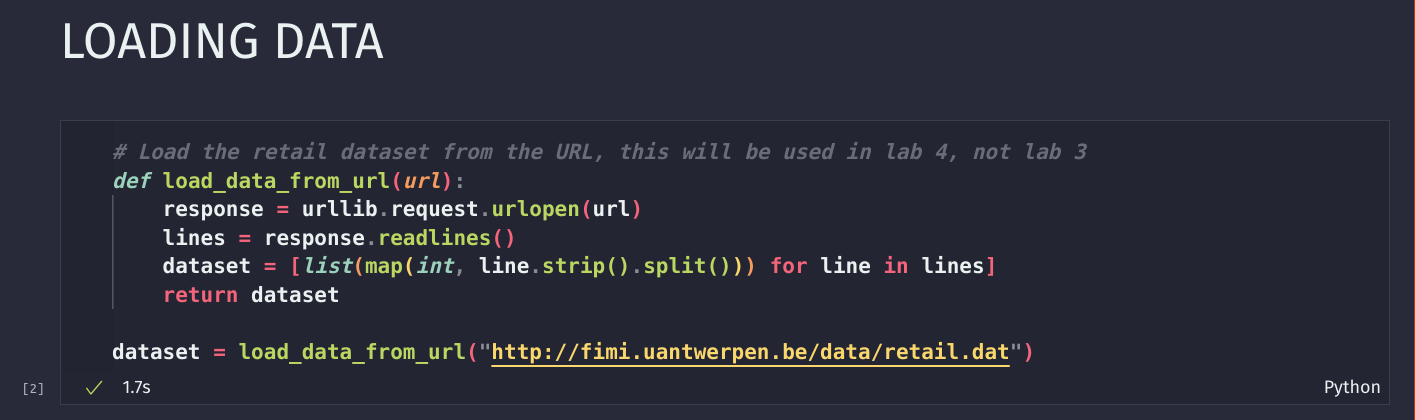
\includegraphics[width=1\textwidth, height=0.2\textheight]{./b.png}
            \end{figure}
        \end{minipage}
        
        \newpage

        \item \begin{minipage}[t]{0.9\textwidth}
            Comparing Apriori and PCY algorithms using the provided partitions
            of the dataset:
            \begin{figure}[H]
                \centering
                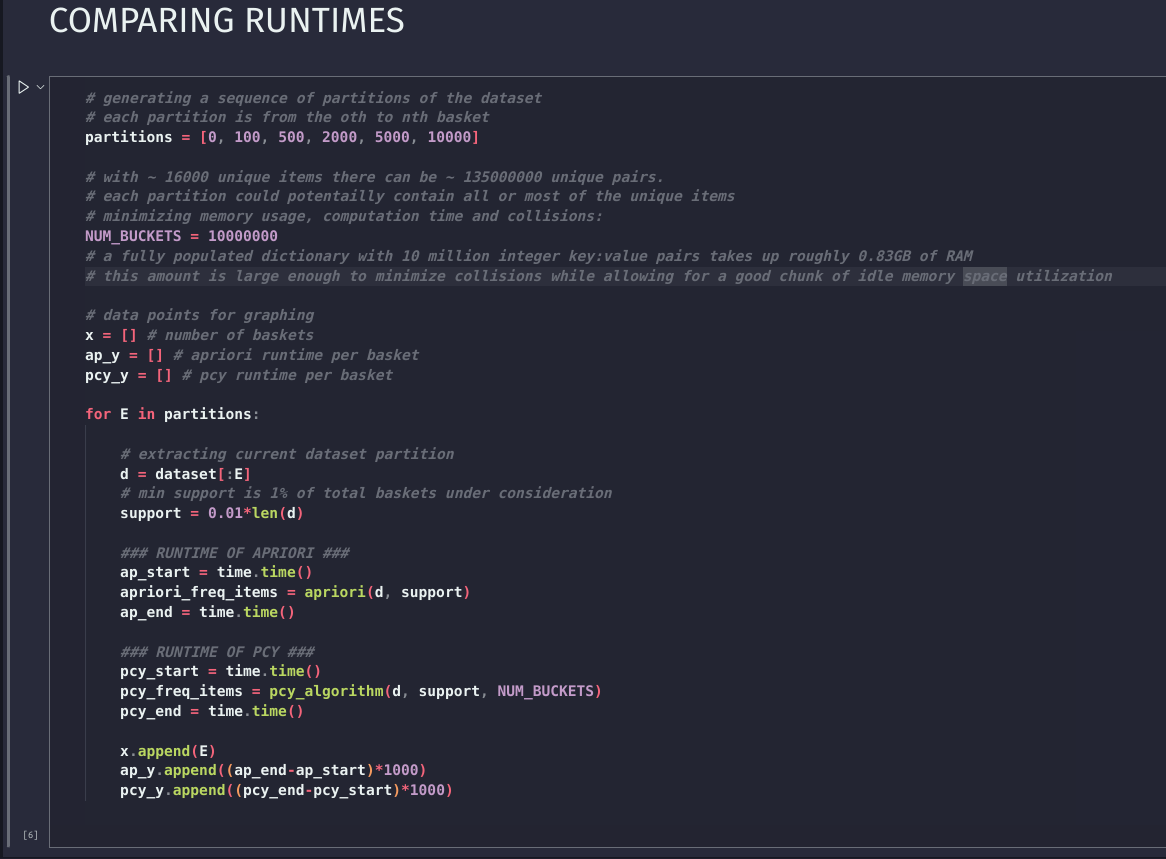
\includegraphics[width=1\textwidth, height=0.4\textheight]{./c.png}
            \end{figure}
        \end{minipage}

        \item \begin{minipage}[t]{0.9\textwidth}
            Graphing results. Dataset size is on the x-axis while runtime (ms) is on y-axis:
            \begin{figure}[H]
                \centering
                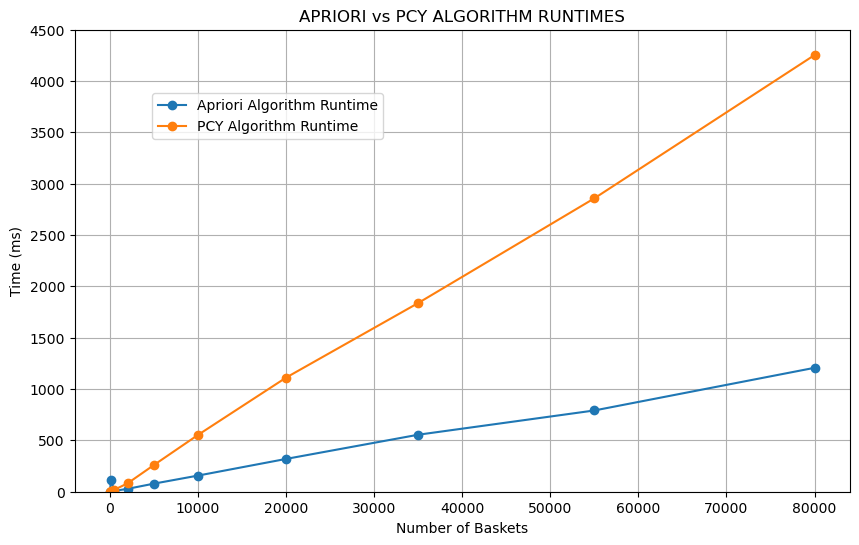
\includegraphics[width=1\textwidth, height=0.4\textheight]{./d.png}
            \end{figure}
        \end{minipage}

        \item \begin{minipage}[t]{0.9\textwidth}
            All screenshots have been provided.
        \end{minipage}
        
        \item \begin{minipage}[t]{0.9\textwidth}
            The runtimes of both Apriori and PCY algorithms seem to increase roughly linearly with
            the size of the dataset. Although the generation and support counting of $k$-tuples for
            each $k$ iteration suggests an exponential increase, the pruning process likely offests
            this cost by greatly reducing the number of candidates to consider. 
            \\\\
            The PCY algorithm is more computationaly expensive then the Apriori algorithm as evident
            by the steeper line in the graph. This faster increase in runtime is due to the
            additional hashing step that is not part of the Apriori algorithm.
            Although more computationaly expensive, the PCY algorithm is less spatially expensive
            thanks to the stringent candidacy requirements it imposes on potential frequent item pairs.
            Because of these requirements, a large number of pairs are pruned from consideration
            freeing up more space in memory.

        \end{minipage}

    \end{enumerate}

    \subsection*{Lab 5} 

    \begin{enumerate}[label=\alph*., left=10pt, itemsep=10pt]

        \item \begin{minipage}[t]{0.9\textwidth}
            The Jaccard similarity of two sets is the size of their intersection divided by the union.
            
            We have the following sets:
            \begin{align*}
                C_{1} &= \{2,3,4,5\}\\
                C_{2} &= \{3,4,6,8\}\\
                C_{3} &= \{2,3,6\}
            \end{align*}
            
            We can now calculate the Jaccard similarity of each pair of the above sets:
            \begin{align*}
                sim(C_{1},C_{2}) &= \frac{|C_{1} \cap C_{2}|}{|C_{1} \cup C_{2}|}\\
                                 &= \frac{|\{2,3,4,5\} \cap \{3,4,6,8\}|}{|\{2,3,4,5\} \cup \{3,4,6,8\}|}\\
                                 &= \frac{|\{3,4\}|}{|\{2,3,4,5,6,8\}|}\\
                                 &= \frac{2}{6}\\
                                 &= \frac{1}{3} = 0.3\overline{3}\\
                \\
                sim(C_{1},C_{3}) &= \frac{|C_{1} \cap C_{3}|}{|C_{1} \cup C_{3}|}\\
                                 &= \frac{|\{2,3,4,5\} \cap \{2,3,6\}|}{|\{2,3,4,5\} \cup \{2,3,6\}|}\\
                                 &= \frac{|\{2,3\}|}{|\{2,3,4,5,6\}|}\\
                                 &= \frac{2}{5} = 0.4\\
                \\
                sim(C_{2},C_{3}) &= \frac{|C_{2} \cap C_{3}|}{|C_{2} \cup C_{3}|}\\
                                 &= \frac{|\{3,4,6,8\} \cap \{2,3,6\}|}{|\{3,4,6,8\} \cup \{2,3,6\}|}\\
                                 &= \frac{|\{3,6\}|}{|\{2,3,4,6,8\}|}\\
                                 &= \frac{2}{5} = 0.4\\
            \end{align*}
            % C_{2} &= \{3,4,6,8\}\\
            % C_{3} &= \{2,3,6\}
        \end{minipage}

    \end{enumerate}

\end{document}